\section{Datenanalyse}
\subsection{Detektor Bilder}
\begin{frame}
	\frametitle{Elektronen Events}
	\begin{minipage}{0.54\linewidth}
		\begin{figure}
			\centering
			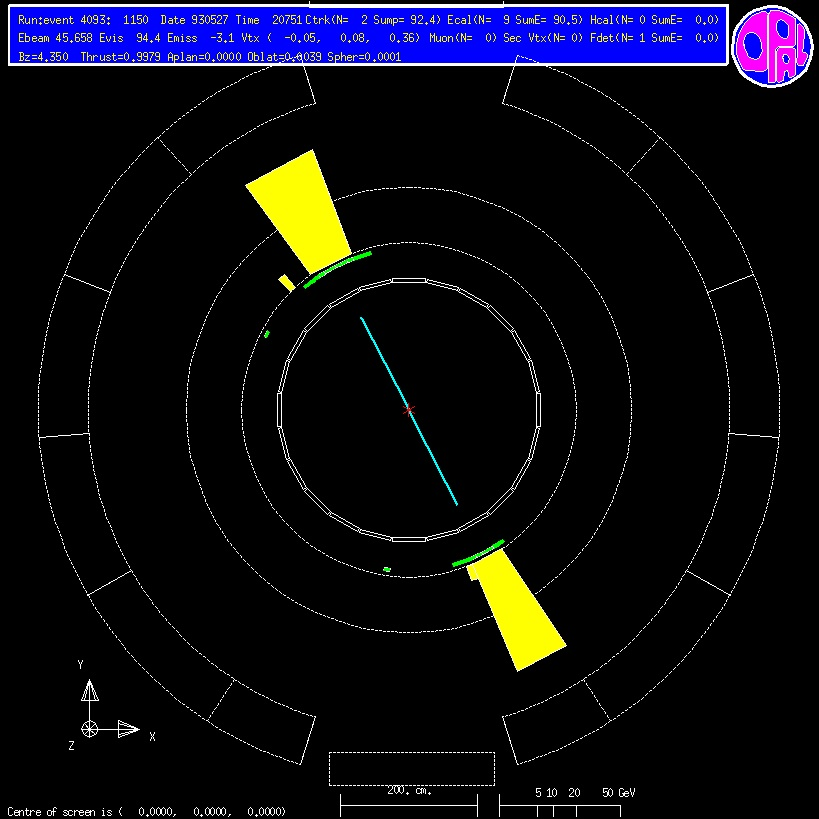
\includegraphics[width=1.0\linewidth]{graphics/electronopal}
		\end{figure}
	\end{minipage}
	\begin{minipage}{0.44\linewidth}
		\begin{center}
			\begin{itemize}
				\item 2 geladene Spuren\\\hfill
				\item Energie in EM-Kalorimeter\\\hfill
			\end{itemize}
		\end{center}
	\end{minipage}
\end{frame}

\begin{frame}
	\frametitle{Myonen Events}
		\begin{minipage}{0.54\linewidth}
			\begin{figure}
				\centering
				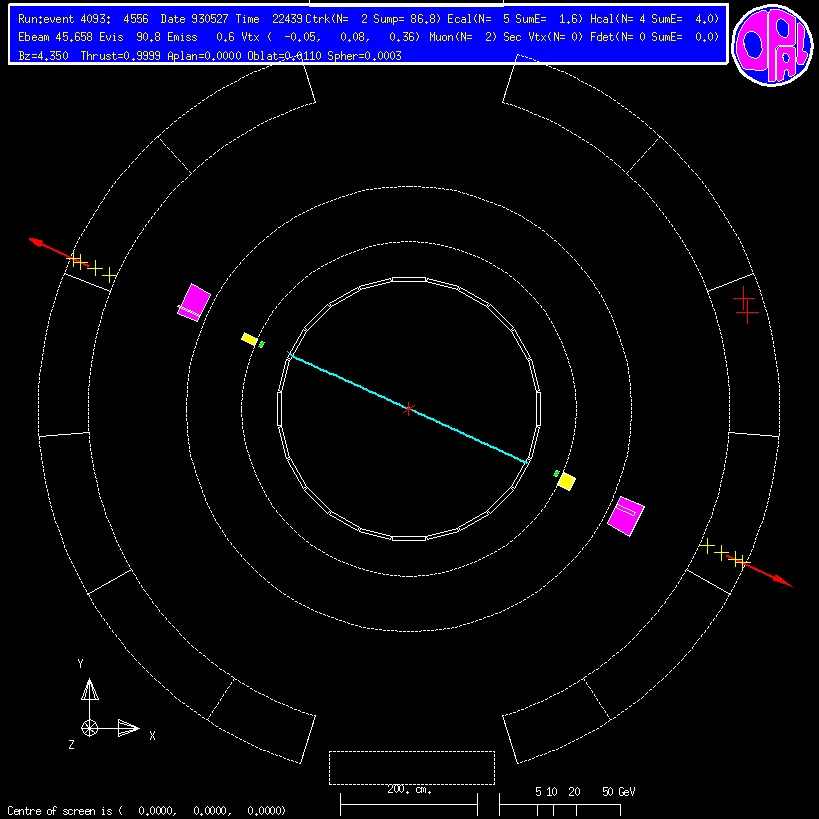
\includegraphics[width=1.0\linewidth]{graphics/muonopal}
			\end{figure}
		\end{minipage}
		\begin{minipage}{0.44\linewidth}
			\begin{center}
				\begin{itemize}
					\item 2 geladene Spuren\\\hfill
					\item Wenig Energie in EM-Kalorimeter\\\hfill
					\item Wenig Energie in Hadronenkalorimeter\\\hfill
					\item Spuren in Myonenkammer
				\end{itemize}
			\end{center}
		\end{minipage}
\end{frame}

\begin{frame}
	\frametitle{Leptonisches Tauonen Event}
		\begin{minipage}{0.54\linewidth}
			\begin{figure}
				\centering
				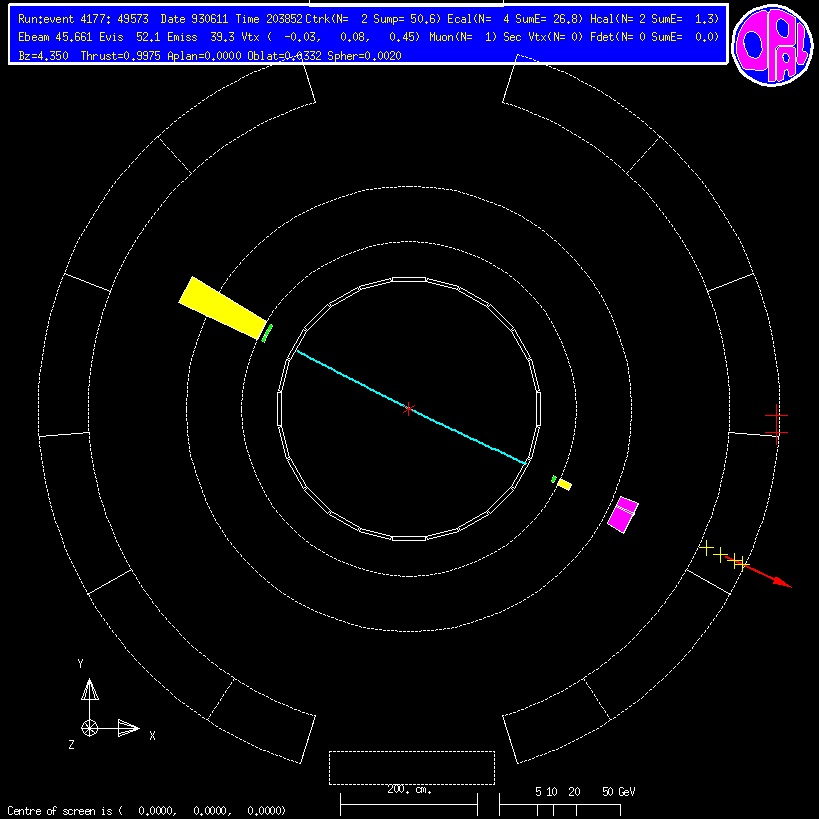
\includegraphics[width=1.0\linewidth]{graphics/tauonopalleptonisch}
			\end{figure}
		\end{minipage}
		\begin{minipage}{0.44\linewidth}
			\begin{center}
				\begin{itemize}
					\item Etwa $\frac{1}{3}$ Wahrscheinlichkeit\\\hfill
					\item 2 geladene Spuren\\\hfill
					\item Ein Myon, ein Elektron\\\hfill
				\end{itemize}
			\end{center}
		\end{minipage}
\end{frame}

\begin{frame}
	\frametitle{Hadronisches Tauonen Event}
		\begin{minipage}{0.54\linewidth}
			\begin{figure}
				\centering
				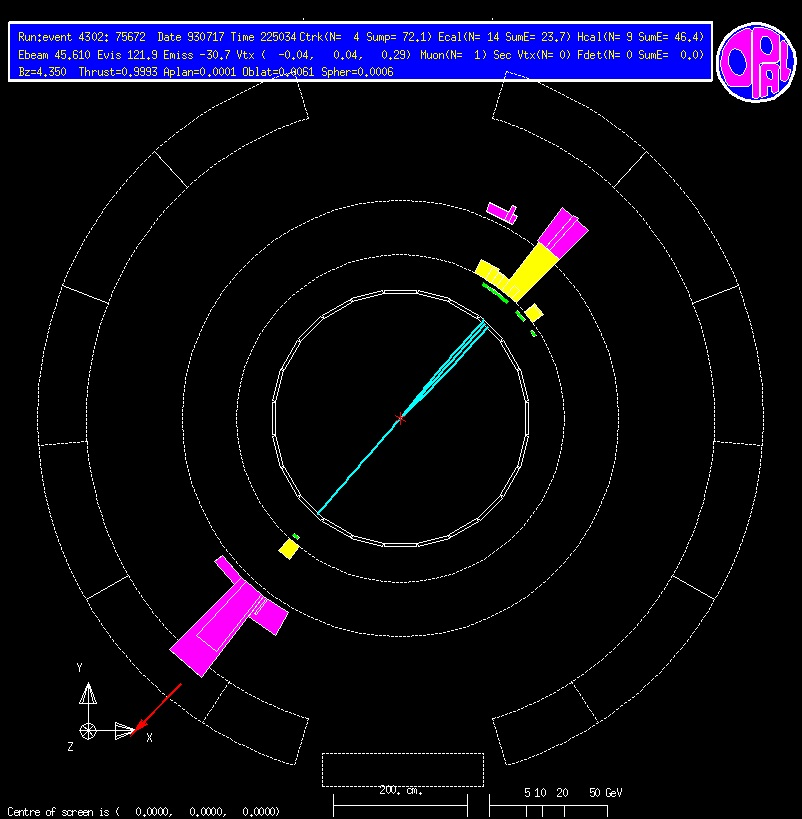
\includegraphics[width=1.0\linewidth]{graphics/tauonopalhadronisch}
			\end{figure}
		\end{minipage}
		\begin{minipage}{0.44\linewidth}
			\begin{center}
				\begin{itemize}
					\item Etwa $\frac{2}{3}$ Wahrscheinlichkeit\\\hfill
					\item Hier zwei mal drei Pionen\\\hfill
					\item Energie in beiden Kalorimetern\\\hfill
				\end{itemize}
			\end{center}
		\end{minipage}
\end{frame}


\begin{frame}
	\frametitle{Quark Events}
		\begin{minipage}{0.54\linewidth}
			\begin{figure}
				\centering
				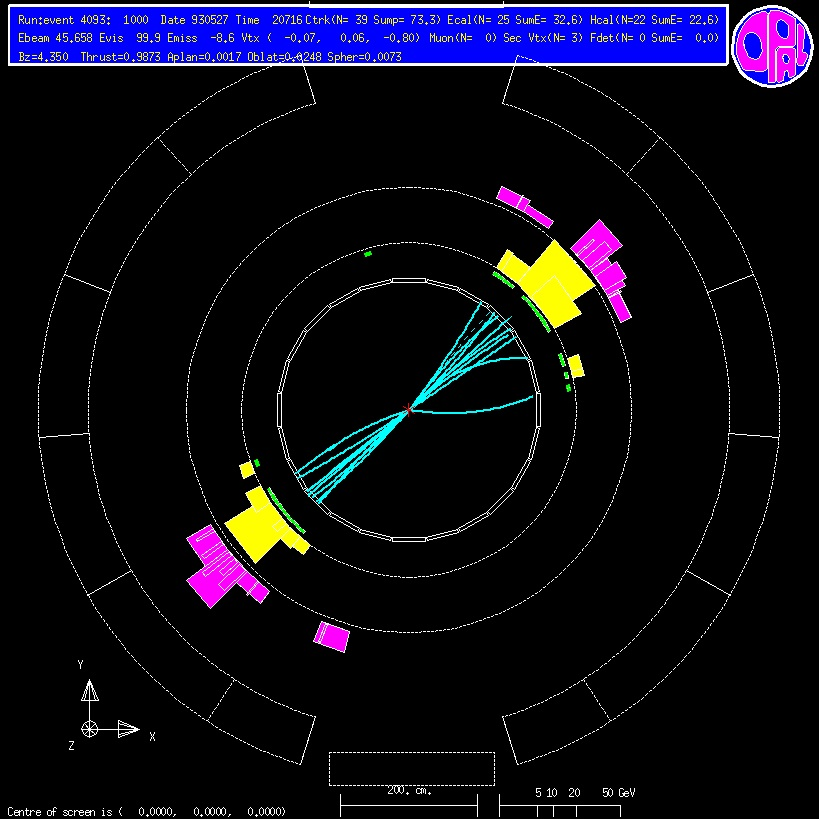
\includegraphics[width=1.0\linewidth]{graphics/quarkopal}
			\end{figure}
		\end{minipage}
		\begin{minipage}{0.44\linewidth}
			\begin{center}
				\begin{itemize}
					\item Ähnlichkeit mit Hadr. Tauonen\\\hfill
					\item Sehr viele Spuren\\\hfill
					\item Energie in beiden Kalorimetern\\\hfill
					\item Beugung der Kurven wegen Magnetfeld
				\end{itemize}
			\end{center}
		\end{minipage}
\end{frame}



\subsection{Cuts und Aufbereitung der Daten}
\begin{frame}
	\frametitle{MC-Simulationen}
	\begin{center}
		\begin{itemize}
			\item Zu viele Events um einzeln zu unterscheiden\\\hfill
			\item Events an Variablen (E\_Ecal, Ncharged...) unterscheiden\\\hfill
			\item MC-Simulation von Events und Detektorsimulation\\\hfill
			\item Daraus Weg finden, Events zu trennen
		\end{itemize}
	\end{center}	
\end{frame}
\begin{frame}
	\frametitle{Energie im EM Kalorimeter}
	\begin{figure}
		\centering
		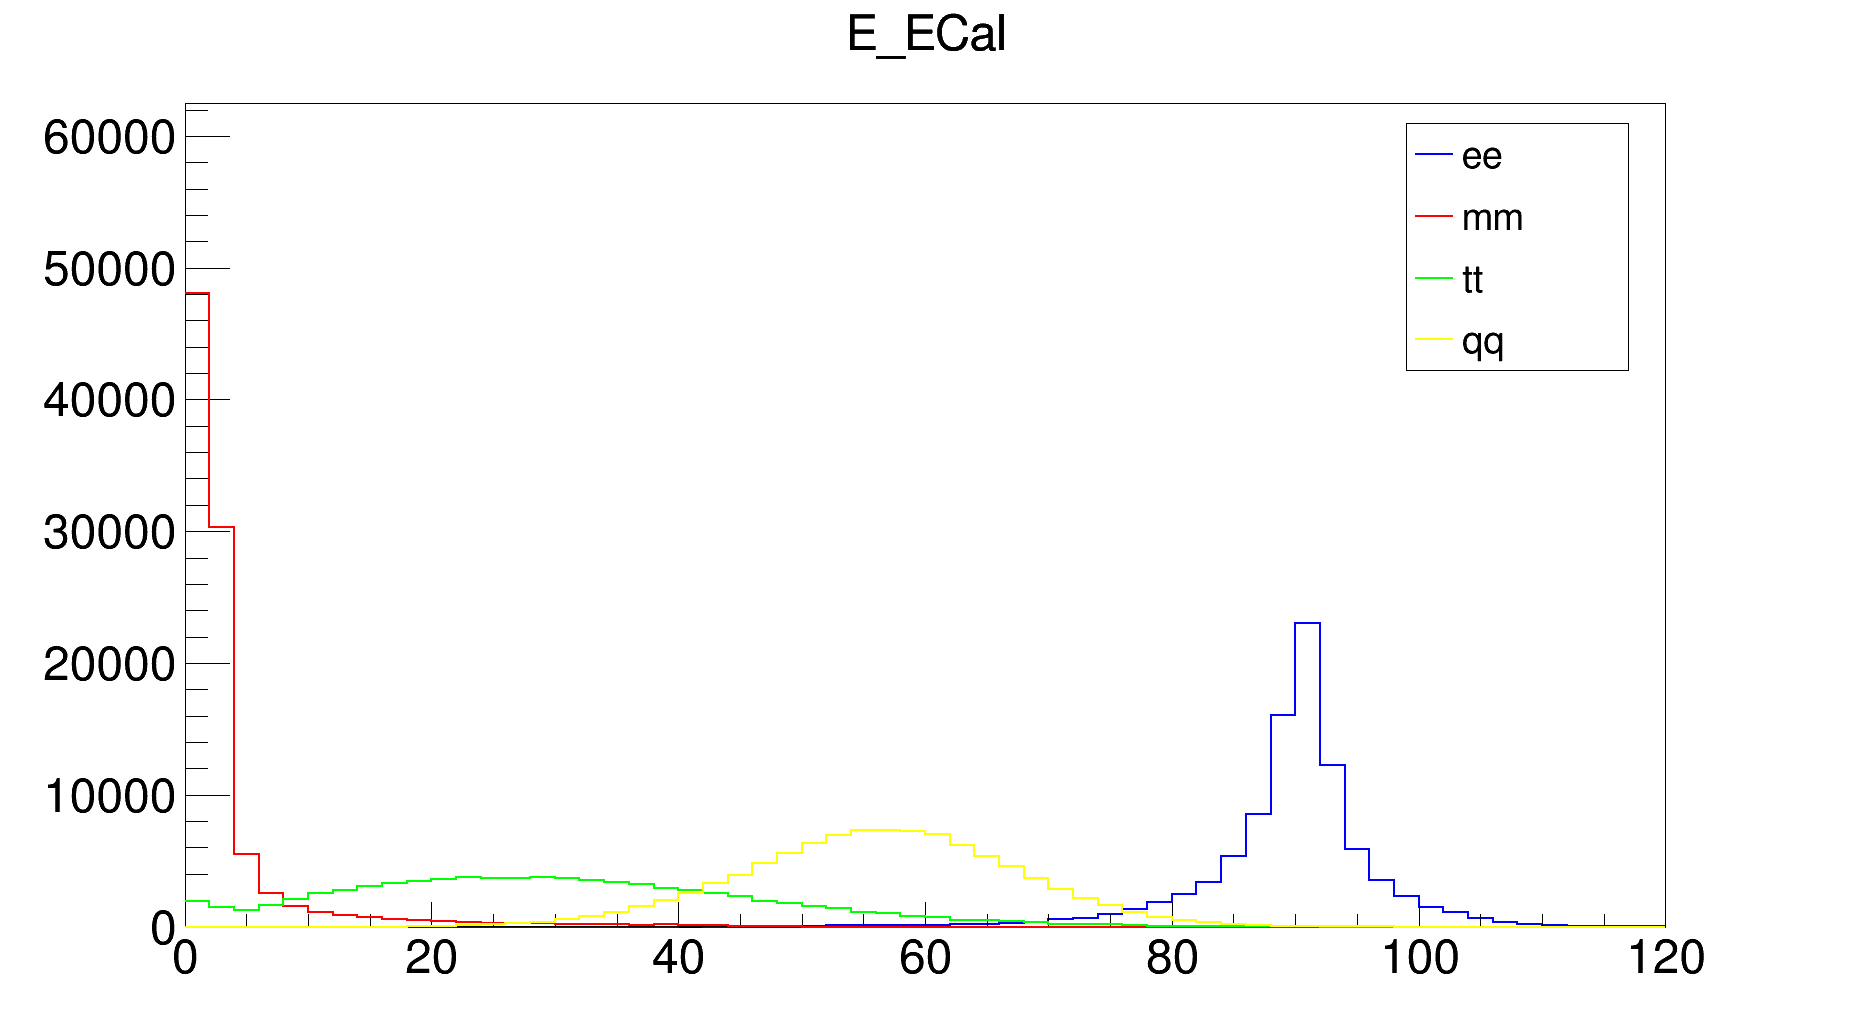
\includegraphics[width=0.9\linewidth]{../results/MC_results/nocut/E_Ecal}
	\end{figure}
	\begin{center}
		\begin{itemize}
			\item \makebox[3cm][l]{\textbf{Elektronen Cut:}} $\ge 70 \unit{GeV}$
			\item \makebox[3cm][l]{\textbf{Myonen Cut:}} $< 50 \unit{GeV}$
			\item \makebox[3cm][l]{\textbf{Tauonen Cut:}} $< 60 \unit{GeV}$
		\end{itemize}
	\end{center}
\end{frame}

\begin{frame}
	\frametitle{Anzahl der geladenen Spuren}
	\begin{figure}
		\centering
		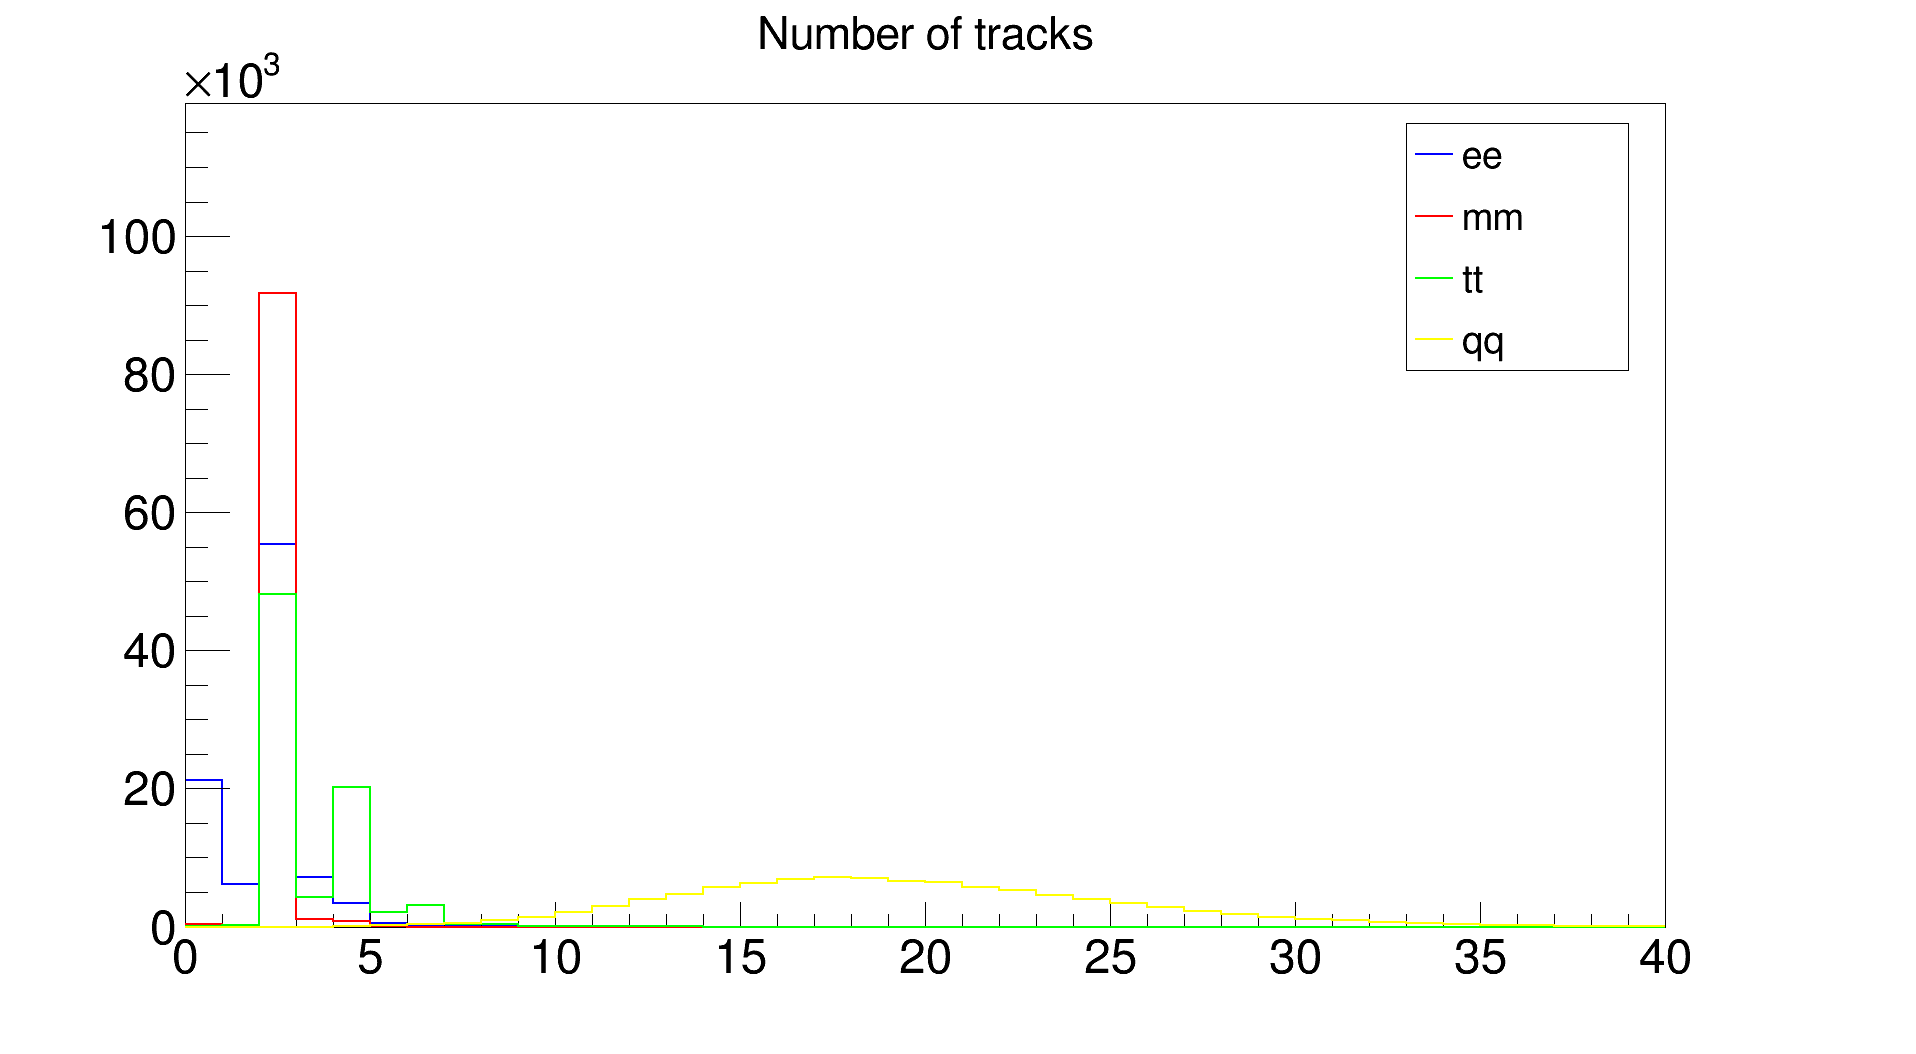
\includegraphics[width=0.85\linewidth]{../results/MC_results/nocut/Ncharged}
	\end{figure}
	\begin{center}
		\begin{itemize}
			\item \makebox[3cm][l]{\textbf{Elektronen Cut:}} $<7$
			\item \makebox[3cm][l]{\textbf{Myonen Cut:}} $=2$
			\item \makebox[3cm][l]{\textbf{Tauonen Cut:}} $<7$
			\item \makebox[3cm][l]{\textbf{Quark Cut:}} $\ge8$
		\end{itemize}
	\end{center}
\end{frame}

\begin{frame}
	\frametitle{Vorher-Nacher Vergleich}
	\begin{minipage}{0.48\linewidth}
			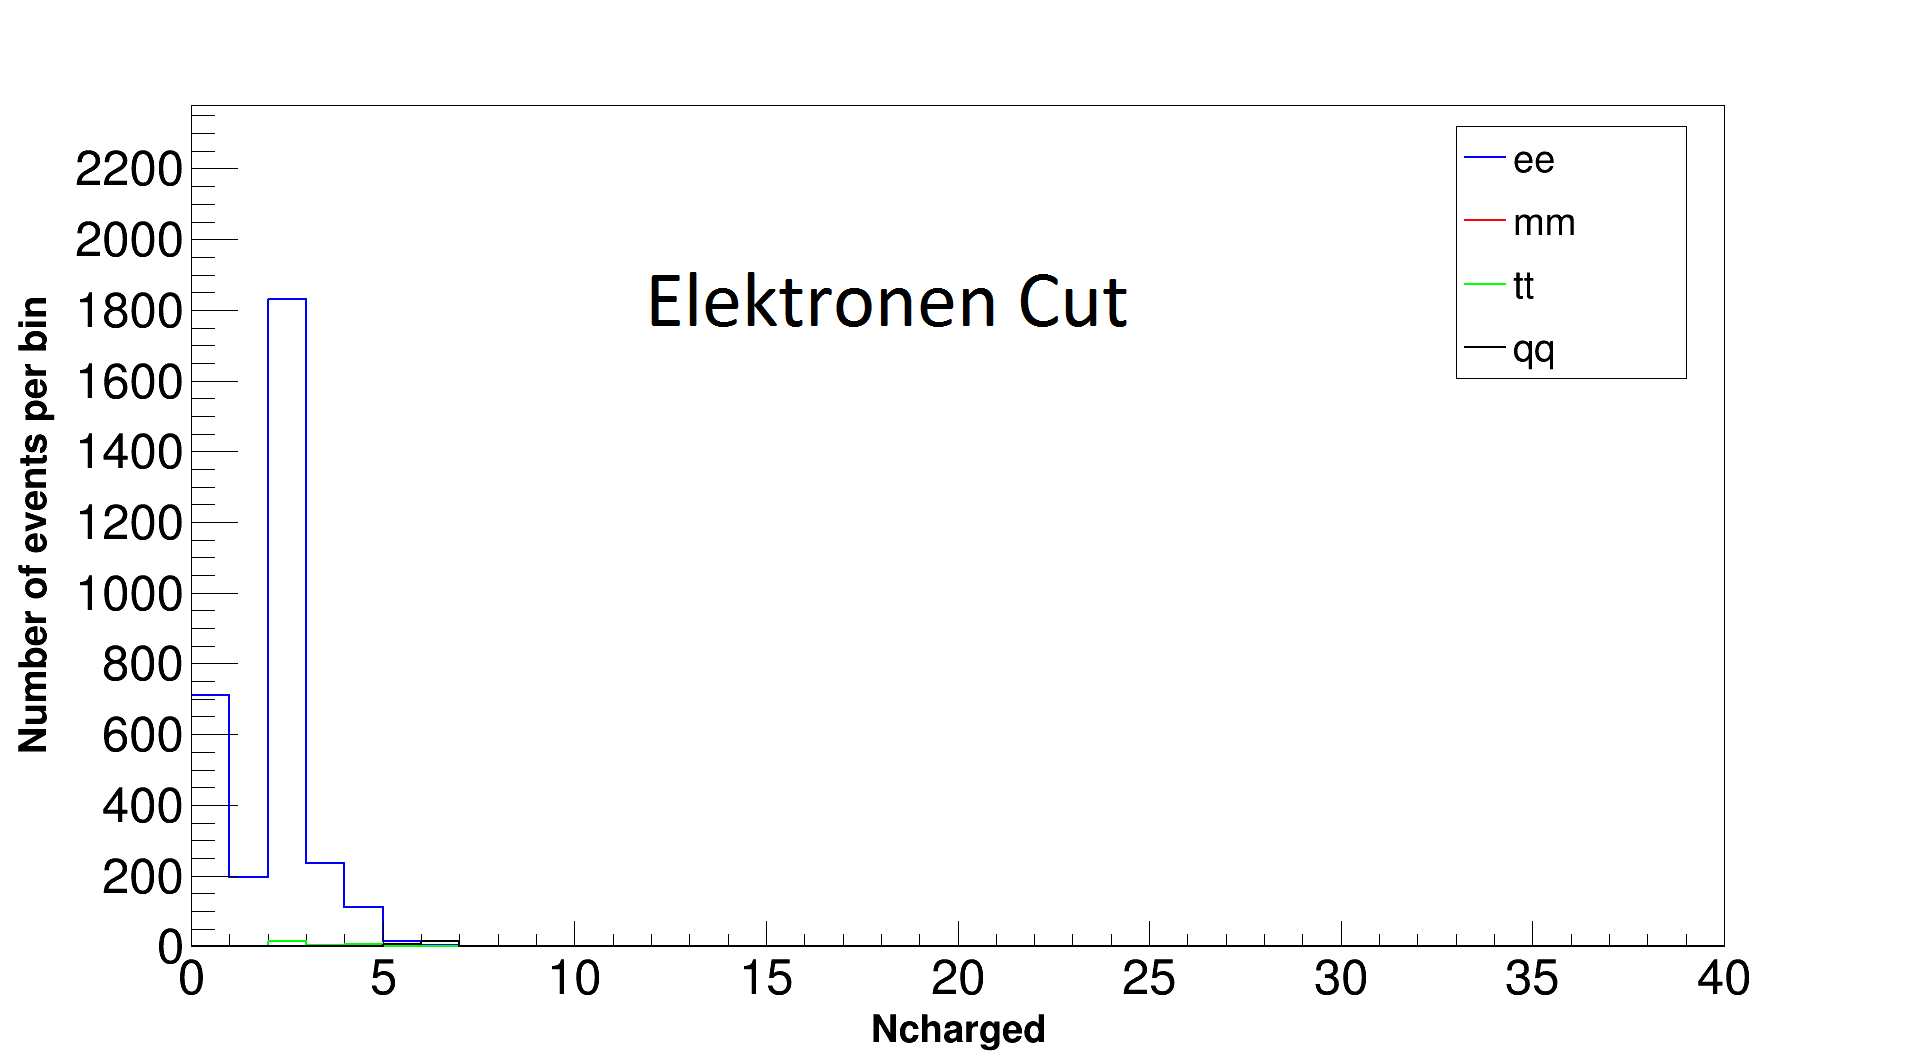
\includegraphics[width=1.1\linewidth]{graphics/Ncharged_vergleich_ee}\\
			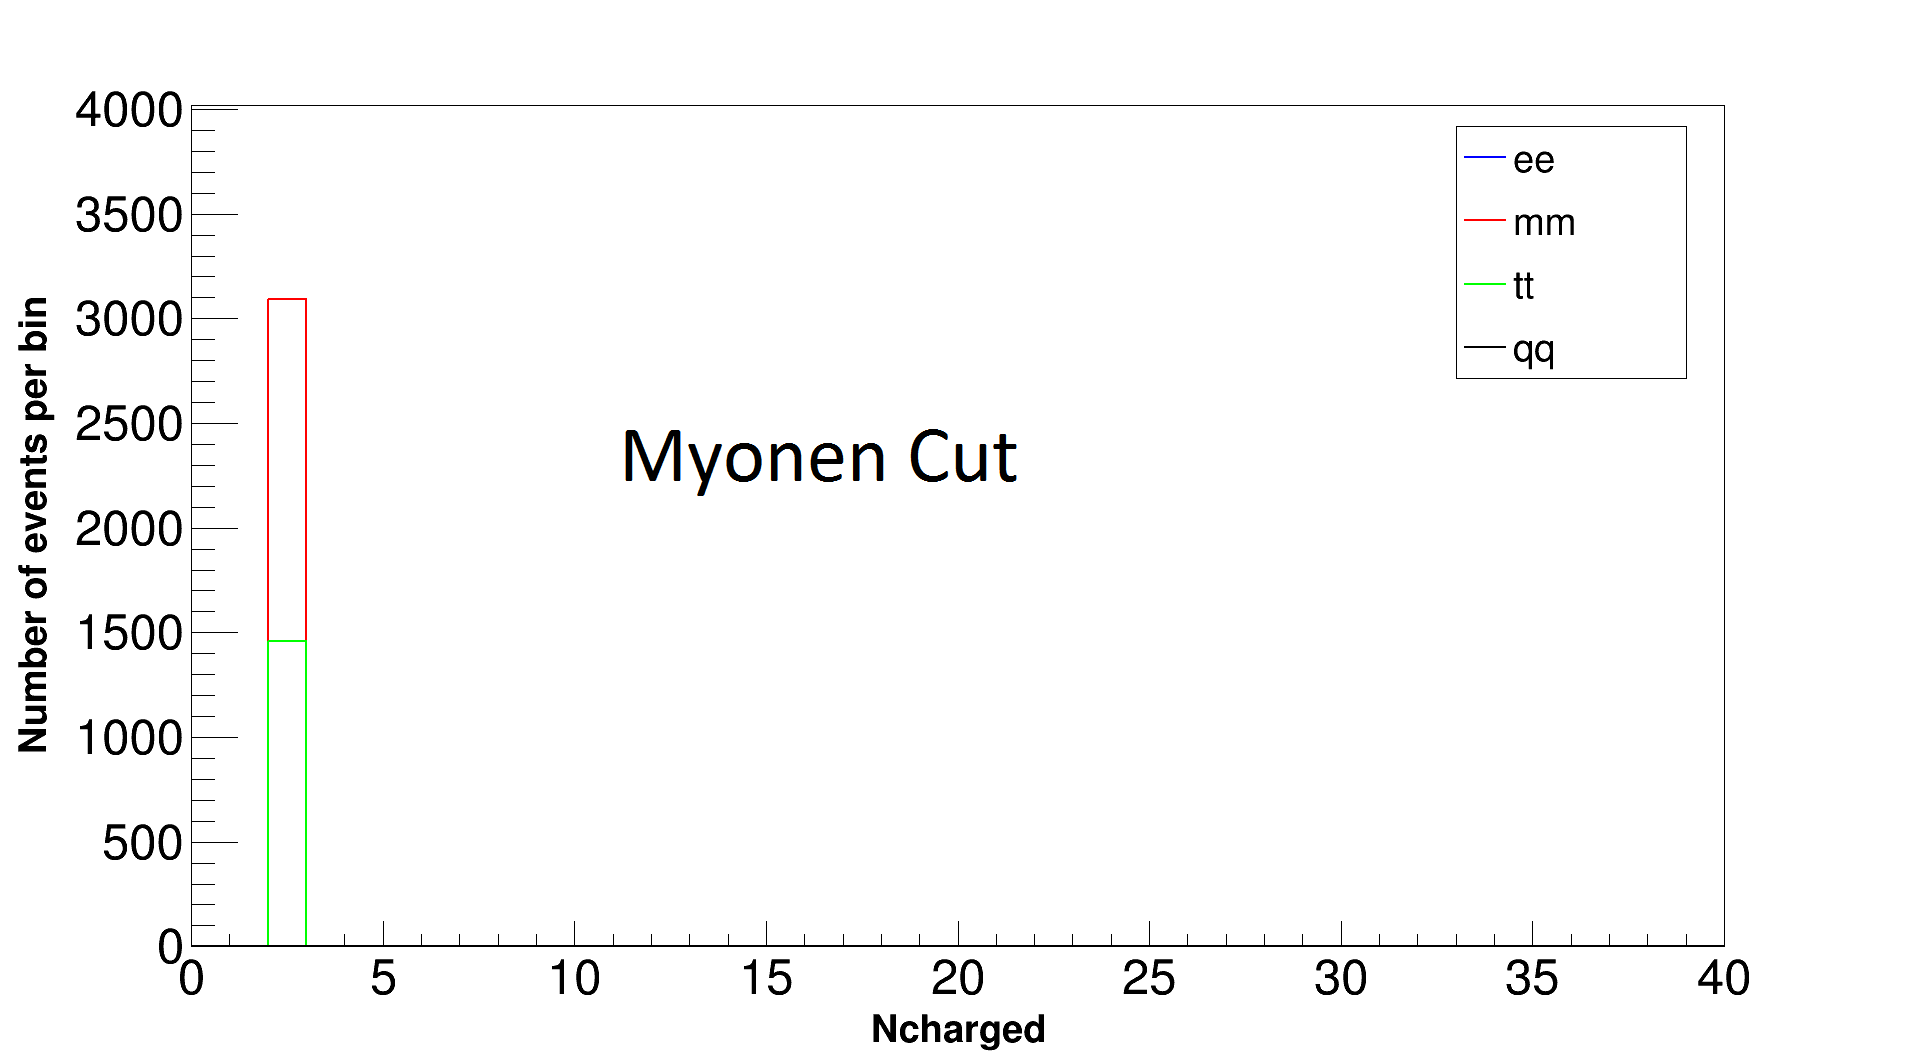
\includegraphics[width=1.1\linewidth]{graphics/Ncharged_vergleich_mm}
	\end{minipage}
	\begin{minipage}{0.48\linewidth}
			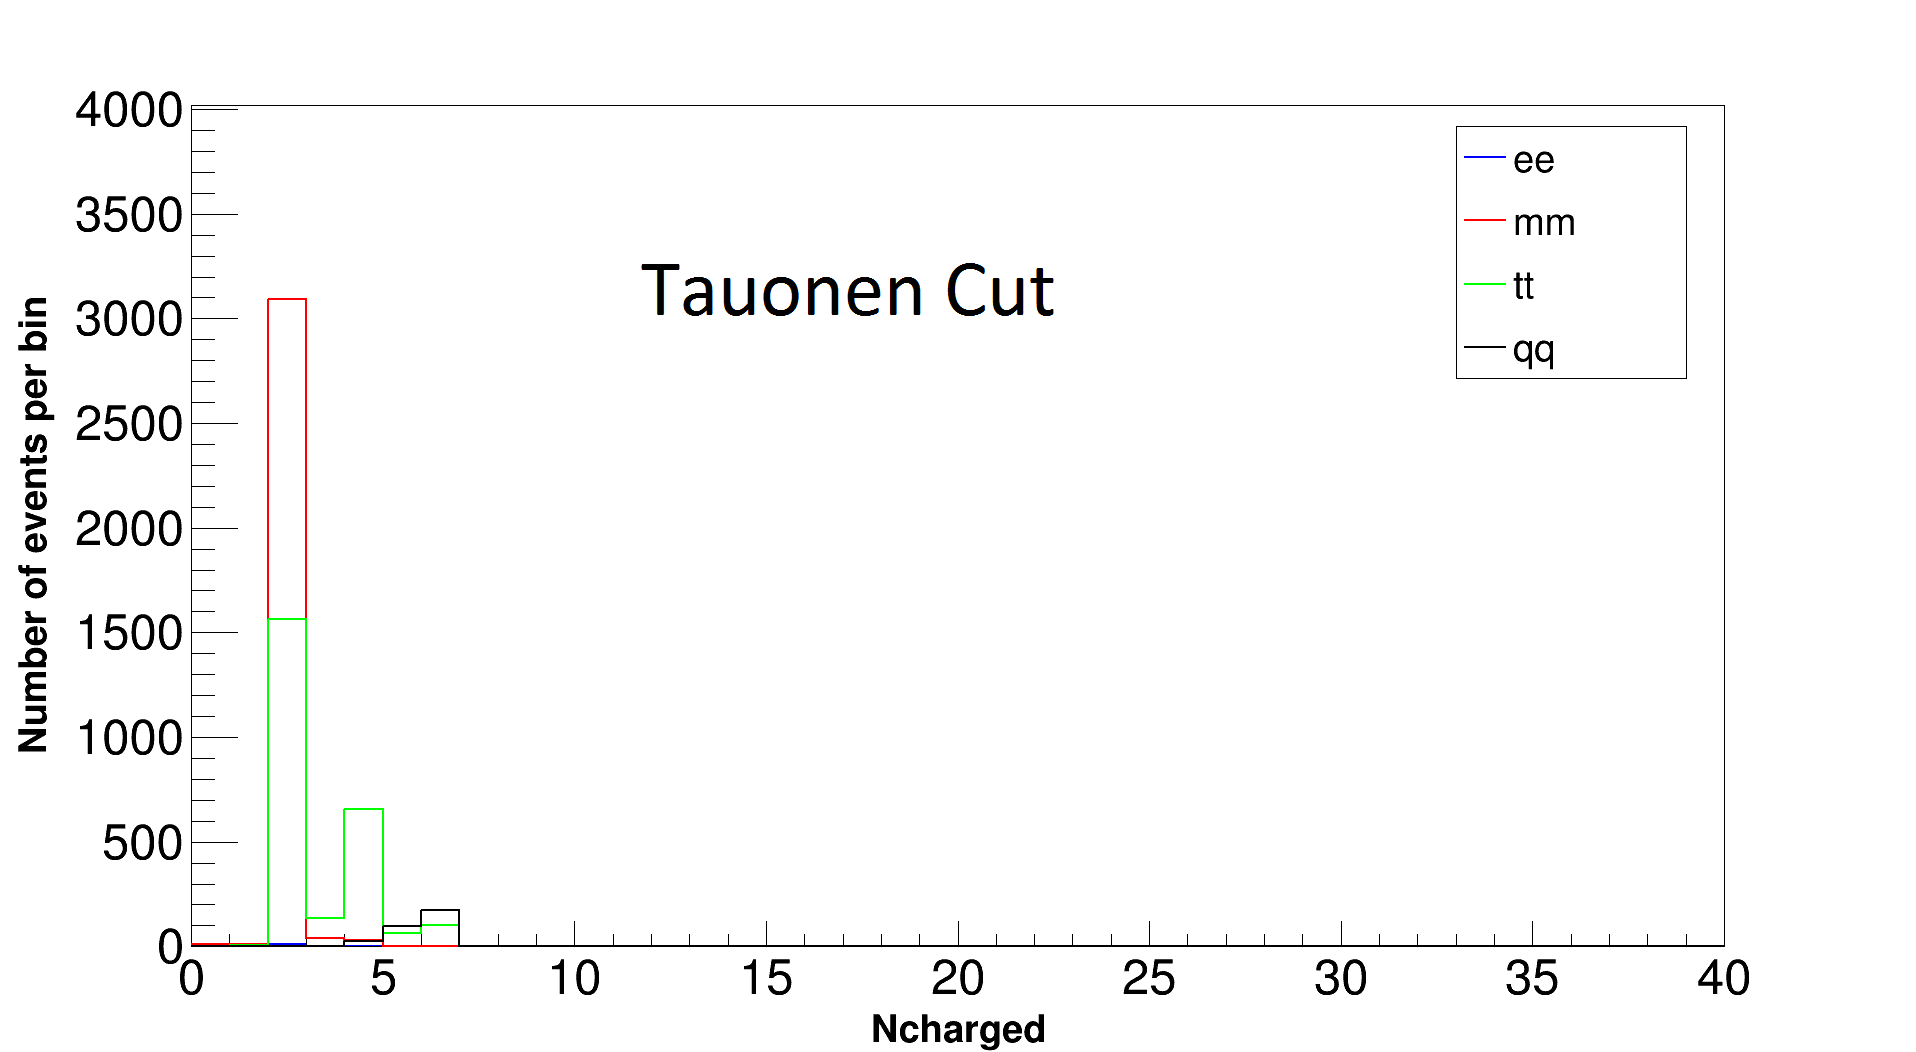
\includegraphics[width=1.1\linewidth]{graphics/Ncharged_vergleich_tt}\\
			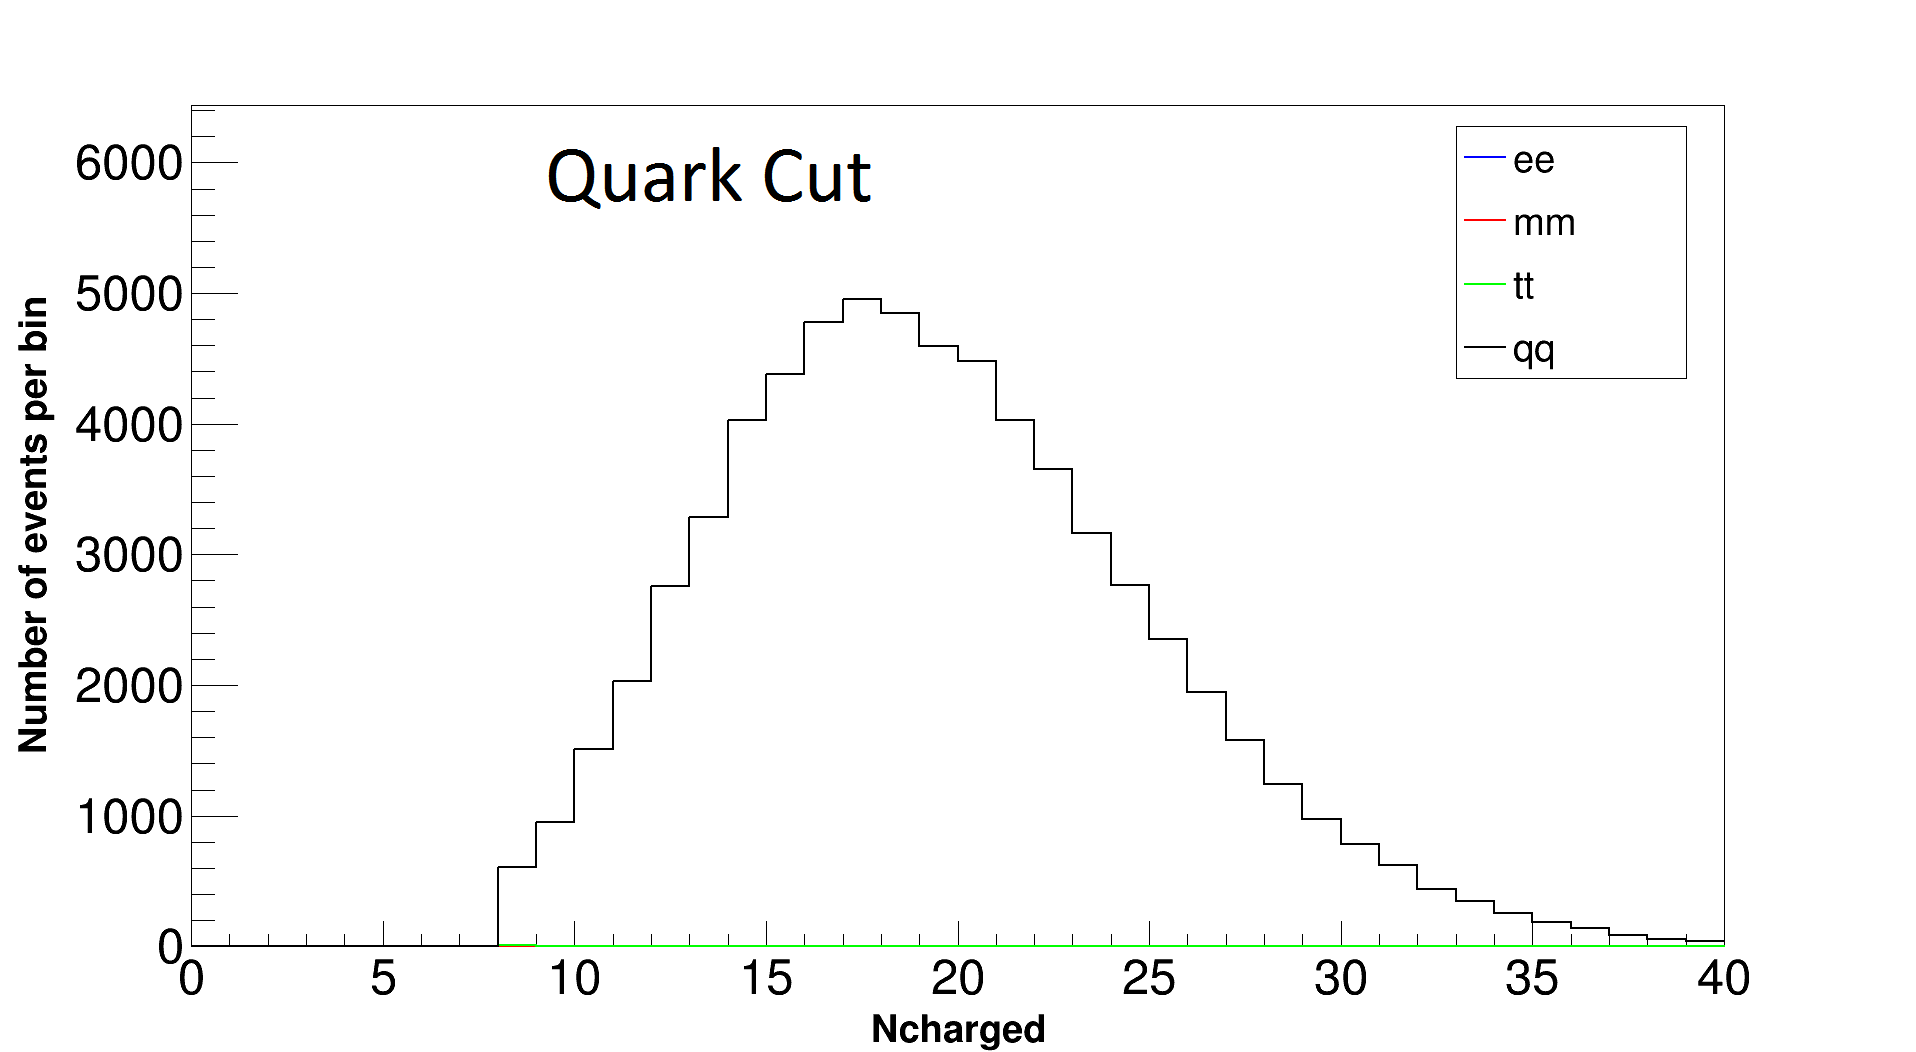
\includegraphics[width=1.1\linewidth]{graphics/Ncharged_vergleich_qq}
		\end{minipage}
\end{frame}
\begin{frame}
	\frametitle{Übersicht über die Cuts}
	\begin{table}[H]\centering
		\begin{tabular}{@{}llllll@{}}
			\toprule
			&			&Ncharged	&Pcharged [GeV]	&E\_Ecal [GeV] &Cos\_theta\\ 
			\midrule
			&$e^+e^-$	&$<7$		&				&$\ge70$		&$\ge-0.9$ \& $\le0.9$\\
			&$\mu^+\mu^-$		&$=2$			&$>71$		&$<50$			&			\\
			&$\tau^+\tau^-$		&$<7$		&$\le60$			&$<60$			&					\\
			&$q\overline{q}$		&$\ge8$		&				&				&			\\
			\bottomrule
		\end{tabular}
	\end{table}
	\begin{minipage}{0.48\linewidth}
		\centering
		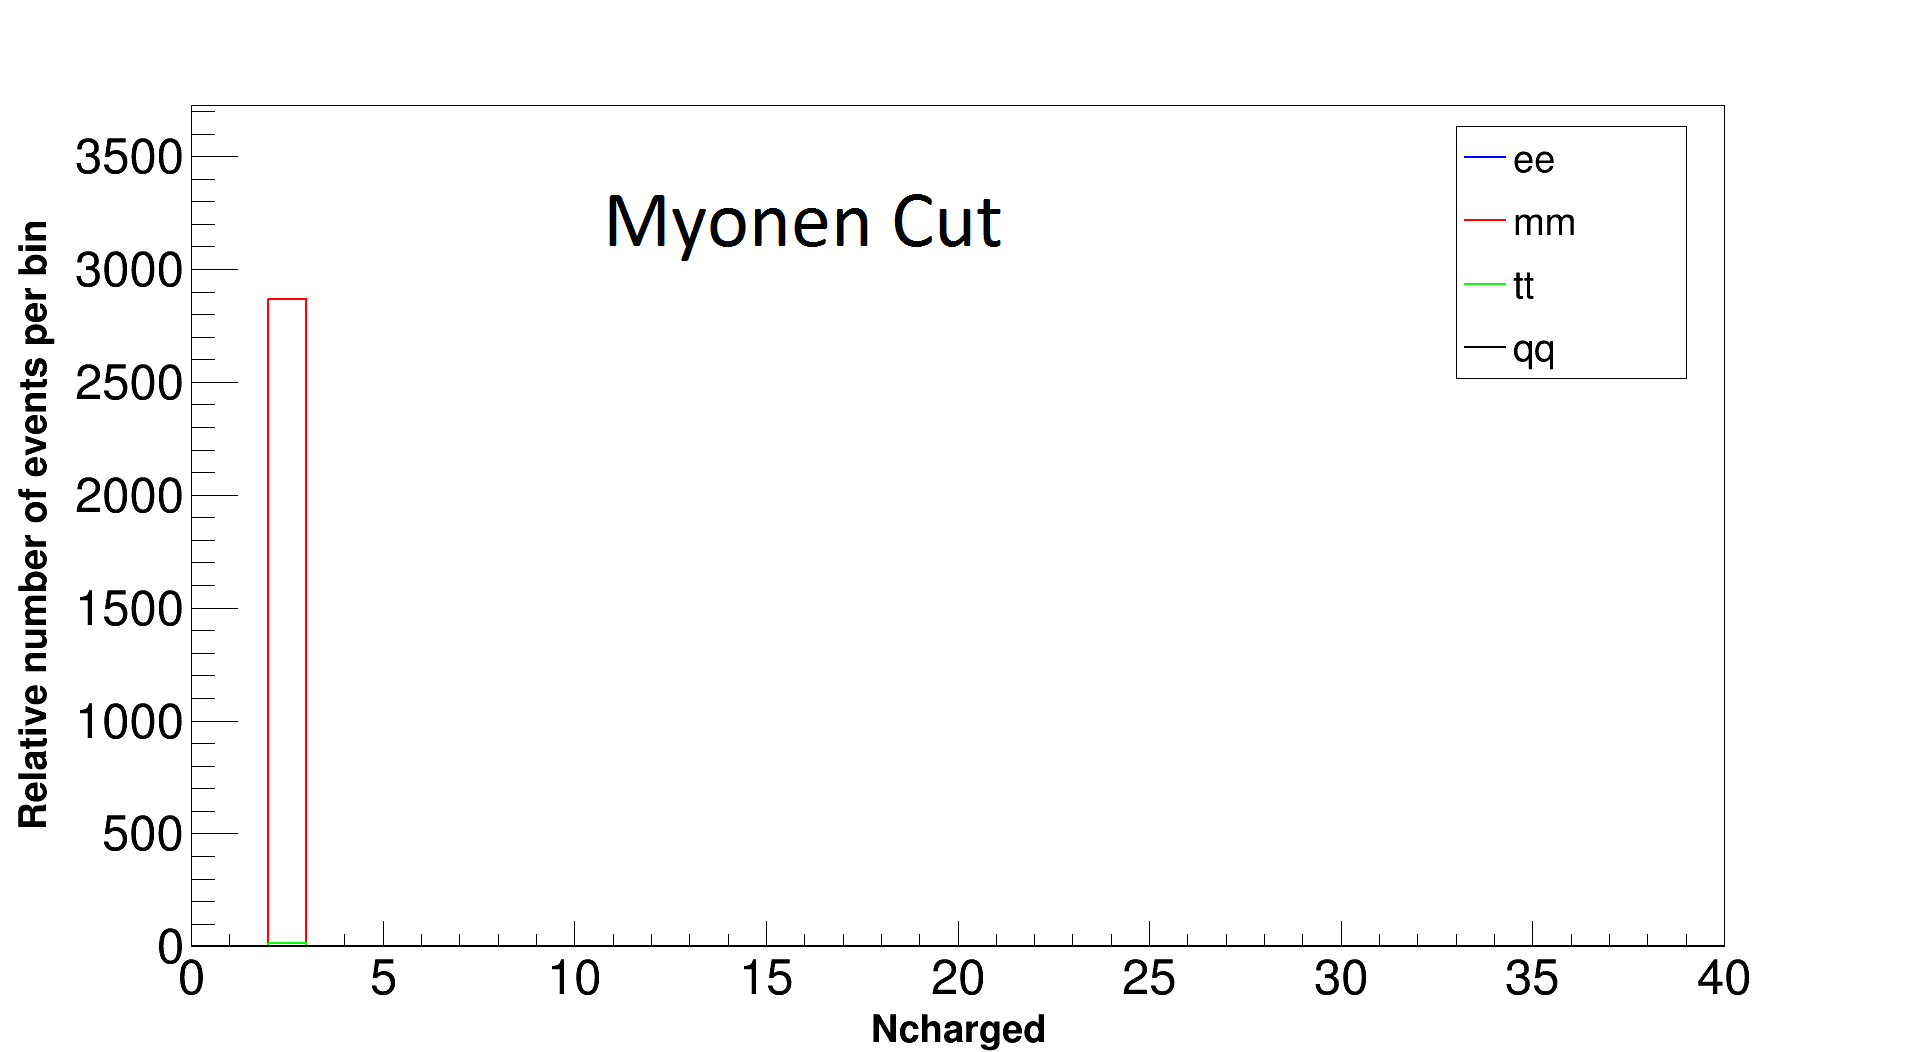
\includegraphics[width=1.1\linewidth]{graphics/Ncharged_final_mm}
	\end{minipage}
	\begin{minipage}{0.48\linewidth}
		\centering
		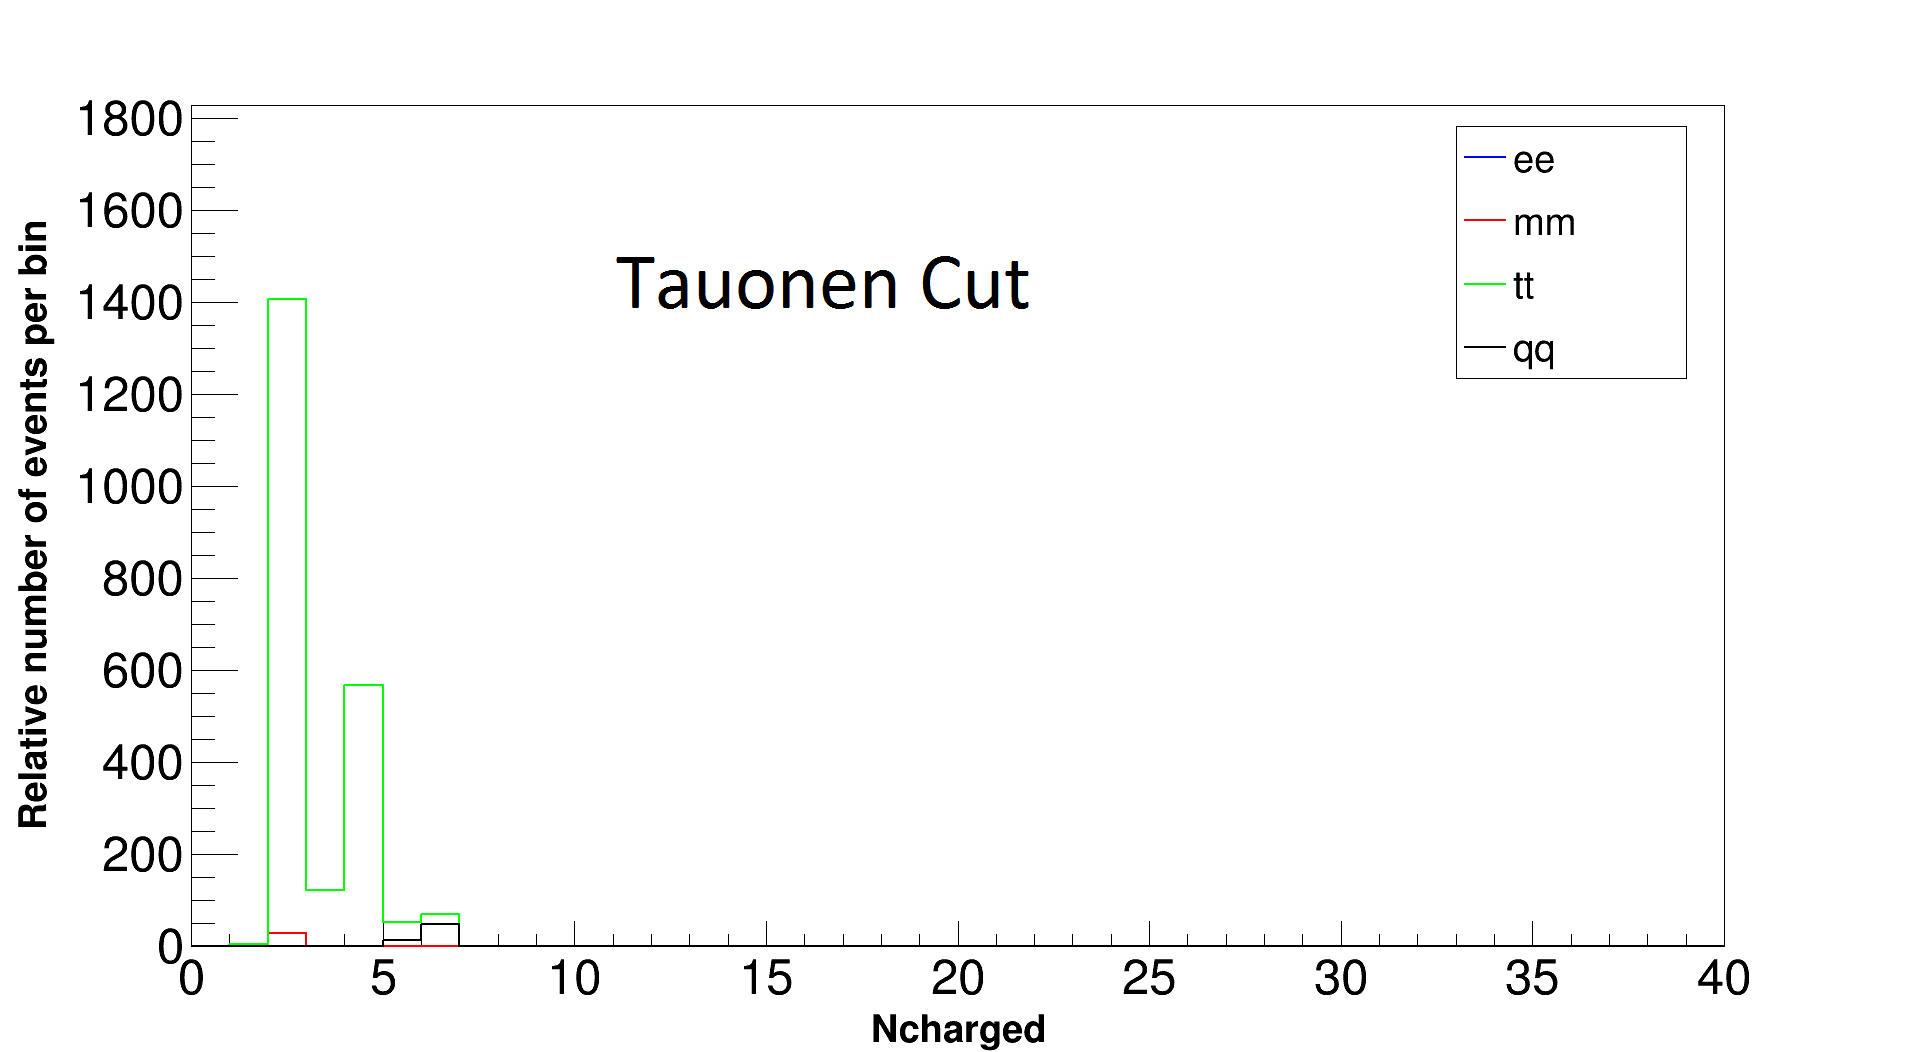
\includegraphics[width=1.1\linewidth]{graphics/Ncharged_final_tt}
	\end{minipage}
\end{frame}
\begin{frame}
	\frametitle{Zwei-Photonen Untergrund}
	\begin{minipage}{0.48\linewidth}
		\centering
		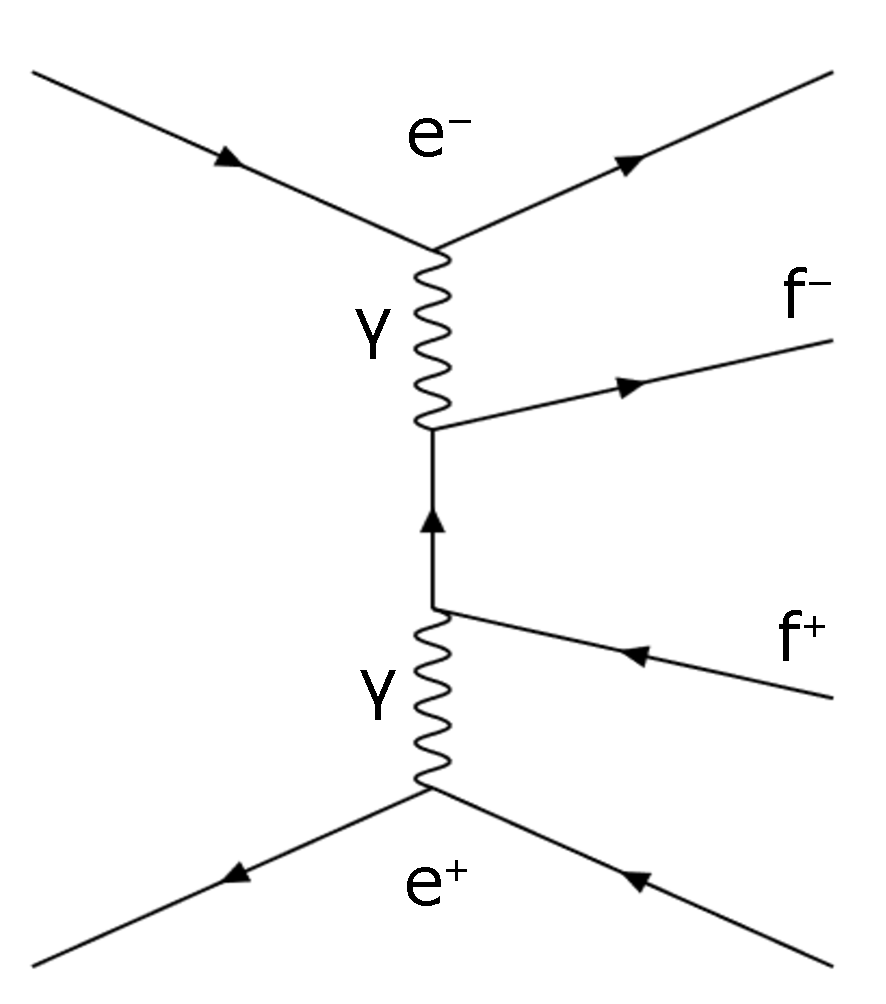
\includegraphics[width=1.0\linewidth]{graphics/twophotonfeynman}
	\end{minipage}
	\begin{minipage}{0.48\linewidth}
		\begin{center}
			\begin{itemize}
				\item Inelastisches Streuungsereignis\\\hfill
				\item Elektronen verlieren wenig Energie\\\hfill
				\item Kein $Z^0$ beteiligt \\$\Rightarrow$ Untergrund\\\hfill
				\item Niederenergetische Fermionen\\ $\Rightarrow$ Zusätzlicher Cut
			\end{itemize}
		\end{center}
	\end{minipage}
\end{frame}


\begin{frame}
	\frametitle{Die Effizienzmatrix}
	Anzahl ausgewählter Elektronenevents:
	\begin{equation*}
	C_e = E_{11} \cdot N_{e} + E_{12} \cdot N_\mu +E_{13} \cdot N_\tau+E_{14} \cdot N_q
	\end{equation*}
	\begin{equation*}
	E_{ij}=\frac{n^{cut}_{ij}}{N_i},\qquad \vec{C}=\boldsymbol{E}\cdot\vec{N}
	\end{equation*}
	\begin{table}[H]\centering
		\begin{tabular}{@{}llllll@{}}
			\toprule
			&Events &$e^+e^-$&$\mu^+\mu^-$&$\tau^+\tau^-$&$q\overline{q}$\\
			\midrule
			&Cut&&&&\\
			&$e^+e^-$&0.39078&0.00002&0.00422&0.00002\\
			&$\mu^+\mu^-$&0.00018&0.90171&0.00611&0.00001\\
			&$\tau^+\tau^-$&0.00039&0.00940&0.83413&0.00094\\
			&$q\overline{q}$&0.00007&0.00001&0.00685&0.98437\\
		\end{tabular}\\
		\noindent\textbox{\hfil Effizienzmatrix\hfil}
	\end{table}
\end{frame}

\begin{frame}
	\frametitle{Reinheit der Cuts}
	\hspace{2cm} Branching Ratios
	\begin{equation*}
		BR_i=\frac{\Gamma_i}{\sum_{j}\Gamma_{j}}
	\end{equation*}
	\hspace{2cm} Reinheit
	\begin{equation*}
		P_i=\frac{BR_i\cdot E_{ii}/N_i}{\sum_{j}BR_j\cdot E_{ij}/N_j}
	\end{equation*}
	\begin{table}\centering
		\begin{tabular}{@{}lll@{}}
			\toprule
			&Cut&Purity\\
			\midrule
			&$e^+e^-$&0.9882\\
			&$\mu^+\mu^-$&0.9928\\
			&$\tau^+\tau^-$&0.9661\\
			&$q\overline{q}$&0.9997\\
			\bottomrule
		\end{tabular}
	\end{table}
\end{frame}

\begingroup
\Large
\begin{frame}
	\frametitle{Die Inverse Effizienzmatrix}
	\hspace{2cm} Eigentliche Anzahl gesucht:
	\begin{equation*}
		\vec{N}=\boldsymbol{E}^{-1}\cdot\vec{C}=:\boldsymbol{I}\cdot\vec{C}
	\end{equation*}
	\hspace{2cm} Toy Experiments:
	\begin{equation*}
		E^{k}_{ij}=E_{ij}+G^k\cdot s_{E_{ij}}
	\end{equation*}
\end{frame}
\endgroup

\begin{frame}
	\frametitle{s-t-Kanal Trennung}
	\begin{figure}
		\centering
		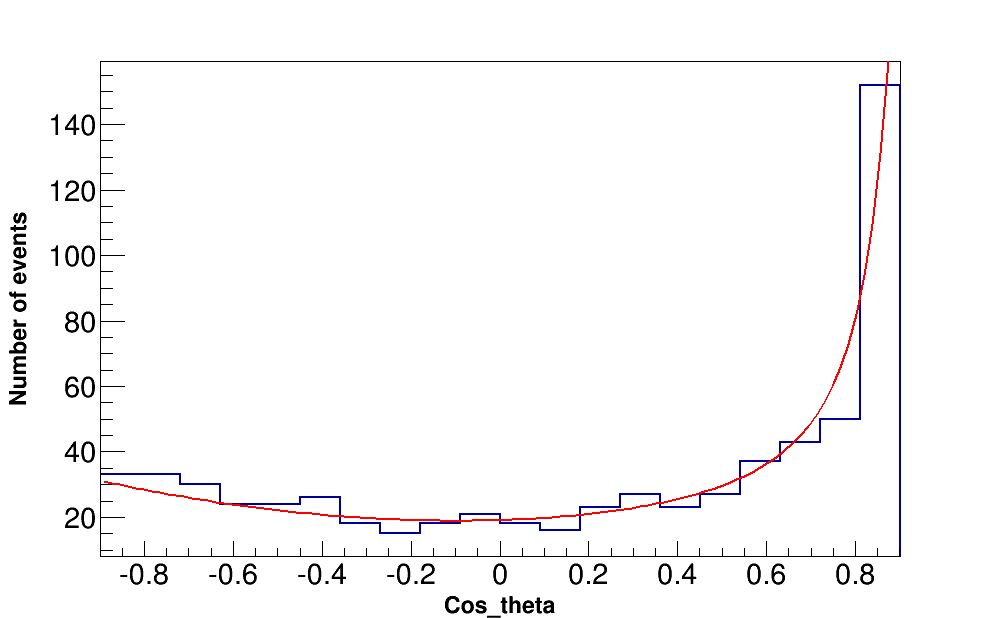
\includegraphics[width=0.85\linewidth]{../results/data_results/cosp_fits/stchannelexample46.png}
	\end{figure}
	\hspace{2cm} Fit Funktion (x=cos\_theta)
	\begin{equation*}
		N(x)=A_s\cdot(1-x^2)+A_t\cdot(1-x)^{-2}
	\end{equation*}
\end{frame}

\begin{frame}
	\frametitle{Berechnung des Korrekturfaktors}
	\begin{equation*}
		c_{st}=\frac{A_s\int_{-0.9}^{0.9}(1+x^2)dx}{A_s\int_{-0.9}^{0.9}(1+x^2)dx+A_t\int_{-0.9}^{0.9}(1-x)^{-2}dx}
	\end{equation*}\\
	\hfill\\
	\hspace{2cm} Integrale sind konstant
	\begin{align*}
		\int_{-0.9}^{0.9}(1+x^2)dx&=2.286\\
		\int_{-0.9}^{0.9}(1-x)^{-2}dx&=9.474
	\end{align*}
\end{frame}

\subsection{Auswertung der aufgearbeiteten Daten}
\begin{frame}
	\frametitle{Wirkungsquerschnitte Elektronen Cut}
	\centering
	\includegraphics[width=0.90\linewidth]{../results/data_results/wqs/WQee}
	\begin{equation*}
	\sigma_i=\frac{N_i}{L}+c_{beam,i}
	\end{equation*}
\end{frame}
\begin{frame}
	\frametitle{Wirkungsquerschnitte Tauonen Cut}
	\centering
	\includegraphics[width=0.90\linewidth]{../results/data_results/wqs/WQtt}
	\begin{itemize}
		\item Elektronen und Taunen Ergebnis nicht in Übereinstimmung mit theoretischem Wert
	\end{itemize}
\end{frame}
\begin{frame}
	\frametitle{Wirkungsquerschnitte Myonen Cut}
	\centering
	\includegraphics[width=0.90\linewidth]{../results/data_results/wqs/WQmm}
	\begin{itemize}
		\item Myonen Ergebnis entspricht Erwartung, in weiteren Rechnungen\\ \noindent\textbox{\hfil$\Gamma_l=\Gamma_\mu$\hfil}
	\end{itemize}
\end{frame}
\begin{frame}
	\frametitle{Wirkungsquerschnitte Quark Cut}
	\centering
	\includegraphics[width=0.90\linewidth]{../results/data_results/wqs/WQqq}
	\begin{equation*}
		\Gamma_q=\frac{\Gamma_f^2}{\Gamma_\mu}=(1777\pm41)\unit{MeV}
	\end{equation*}
\end{frame}
\begin{frame}
	\frametitle{Zerfallsbreiten und Leptonenuniversalität}
	\mbox{}\\
	\begin{equation*}
	\sigma(s) = \frac{12\pi}{ \tikzmark{MZ1}M_Z^2}\frac{s\cdot \tikzmark{gammaf}\Gamma_f^2}{(s-\tikzmark{MZ2}M_Z^2)^2+s^2\cdot\tikzmark{gammaZ}\Gamma_Z^2 / \tikzmark{MZ3}M_Z^2}
	\end{equation*}
	\begin{tikzpicture}[
	remember picture,
	overlay,
	expl1/.style={draw=orange,fill=orange!30,rounded corners},
	expl2/.style={draw=gray!20,fill=gray!10,rounded corners},
	arrow1/.style={red!80!black,ultra thick,->,>=latex},
	arrow2/.style={gray!20,ultra thick,->,>=latex}
	]
	\node[expl1]
	(gammafexpl)
	at (2,2cm)
	{\textcolor{black}{Zerfallsbreite Fermion}};
	\node[expl2]
	(MZexpl)
	at (1,-1cm)
	{\textcolor{gray}{Masse $Z^0$}};
	\node[expl1]
	(gammaZexpl)
	at (10.5,-1cm)
	{\textcolor{black}{Zerfallsbreite $Z^0$}};
	\draw[arrow1]
	(gammafexpl.east) to[out=0,in=90] ([yshift=19ex,xshift=0.75ex]{pic cs:gammaf});
	\draw[arrow2]
	(MZexpl.east) to[out=0,in=270] ([yshift=17ex,xshift=0.7ex]{pic cs:MZ1});
	\draw[arrow2]
	(MZexpl.east) to[out=0,in=270] ([yshift=17ex,xshift=0.7ex]{pic cs:MZ2});
	\draw[arrow2]
	(MZexpl.east) to[out=0,in=270] ([yshift=17ex,xshift=0.7ex]{pic cs:MZ3});
	\draw[arrow1]
	(gammaZexpl.west) to[out=180,in=270] ([yshift=17ex,xshift=0.5ex]{pic cs:gammaZ});
	\end{tikzpicture}
	\mbox{}\\\mbox{}\\\mbox{}\\\mbox{}\\
	\begin{table}[h]\centering
		\begin{tabular}{@{}llllll@{}}
			\toprule
			&Event $i$&$\Gamma_{Z}$ [GeV]&$s_{\Gamma_{Z}}$ [GeV]&$\Gamma_i$ [MeV]&$s_{\Gamma_i}$ [MeV]\\
			\midrule
			&$e^+e^-$&2.28&0.11&94&4\\
			&$\mu^+\mu^-$&2.52&0.06&82.9&1.7\\
			&$\tau^+\tau^-$&2.48&0.07&76.9&1.9\\
			&$q\overline{q}$&2.526&0.019&1777&41\\
			\bottomrule
		\end{tabular}
	\end{table}
\end{frame}
\begin{frame}
	\frametitle{Masse des $Z^0$ Bosons}
	\begin{equation*}
		M_{Z^0}=(91.188\pm0.008)\unit{GeV}
	\end{equation*}
	\mbox{}\\\mbox{}\\\mbox{}\\
	\begin{equation*}
		\sigma(s) = \frac{12\pi}{ \tikzmark{MZ1}M_Z^2}\frac{s\cdot \tikzmark{gammaf}\Gamma_f^2}{(s-\tikzmark{MZ2}M_Z^2)^2+s^2\cdot\tikzmark{gammaZ}\Gamma_Z^2 / \tikzmark{MZ3}M_Z^2}
	\end{equation*}
	\begin{tikzpicture}[
	remember picture,
	overlay,
	expl1/.style={draw=orange,fill=orange!30,rounded corners},
	expl2/.style={draw=gray!20,fill=gray!10,rounded corners},
	arrow1/.style={red!80!black,ultra thick,->,>=latex},
	arrow2/.style={gray!20,ultra thick,->,>=latex}
	]
	\node[expl2]
	(gammafexpl)
	at (2,2cm)
	{\textcolor{gray}{Zerfallsbreite Fermion}};
	\node[expl1]
	(MZexpl)
	at (1,-1cm)
	{Masse $Z^0$};
	\node[expl2]
	(gammaZexpl)
	at (10.5,-1cm)
	{\textcolor{gray}{Zerfallsbreite $Z^0$}};
	\draw[arrow2]
	(gammafexpl.east) to[out=0,in=90] ([yshift=2ex,xshift=0.75ex]{pic cs:gammaf});
	\draw[arrow2]
	(gammaZexpl.west) to[out=180,in=270] ([yshift=-1ex,xshift=0.5ex]{pic cs:gammaZ});
	\draw[arrow1]
	(MZexpl.east) to[out=0,in=270] ([yshift=-1ex,xshift=1ex]{pic cs:MZ1});
	\draw[arrow1]
	(MZexpl.east) to[out=0,in=270] ([yshift=-1ex,xshift=1ex]{pic cs:MZ2});
	\draw[arrow1]
	(MZexpl.east) to[out=0,in=270] ([yshift=-1ex,xshift=1ex]{pic cs:MZ3});
	\end{tikzpicture}
	\mbox{}\\\mbox{}\\\mbox{}\\
\end{frame}

\begin{frame}
	\frametitle{Neutrinogenerationen}
	\hspace{2cm} Blinde Zerfallsbreite
	\begin{equation*}
		\Gamma_{blind}=\Gamma_{Z}^{ave}-3\cdot\Gamma_l-\Gamma_{q\overline{q}}=(0.49\pm0.04)\unit{GeV}
	\end{equation*}
	\hspace{2cm} Anzahl Neutrinogenerationen
	\begin{equation*}
		n_{\nu-gen}=\frac{\Gamma_{blind}}{\Gamma_{\nu}^{calc}}=(2.93\pm0.26)
	\end{equation*}
\end{frame}
\begin{frame}
	\frametitle{Vorwärts-Rückwärts Asymmetrie}
	\begin{equation*}
		A_{fb}=\frac{N_f-N_b}{N_f+N_b}
	\end{equation*}
	\begin{table}[h]\centering
		\begin{tabular}{@{}llllll@{}}
			\toprule
			&$\sqrt{s}$ [GeV]&$N_f$&$N_b$&$A_{fb}$&$s_{A_{fb}}$\\
			\midrule
			&89.5&117&112&0.02&0.07\\
			&91.23&1845&1881&\textcolor{red}{-0.010}&0.016\\
			&93.0&153&99&0.21&0.06\\
			\bottomrule
		\end{tabular}
	\end{table}
	\begin{equation*}
	\theta_w\approx\arcsin(\sqrt{\frac{1-\sqrt{A_{fb}/3}}{4}})
	\end{equation*}
\end{frame}




